\documentclass{beamer}
\usepackage{graphicx}
\usepackage{amsmath}
\graphicspath{{./images/}}
\begin{document}
\title{Topological Data Analysis of Images}


\begin{frame}
\titlepage
\end{frame}


\begin{frame}{1. Persistent Homology}
A \textbf{persistence complex} is a sequence of 
chain complexes along with chain maps $x_i : C_*^i \longrightarrow 
C_*^{i+1}$. \break

For $i<j$ the $(i,j)^{th}$ \textbf{persistent homology} of C 
denoted by $H_*^{i \rightarrow j}(C)$ is the image of $i: \ 
H_*(C^i) \longrightarrow H_*(C^j)$.\break

For a finite persistence module over a field, we can use the 
structure theorem over PID to interpret the homology module 
$H_*(C;F)$. The free part is in correspondence with homology 
generators that appear at a specific value and 
persist forever, while the torsion part is in correspondence 
with homology parameters that appear at a particular value and 
disappear at a higher value. \break

Thus, the parameter intervals arising from basis for $H_*(C;F)
$ in structure theorem can be represented as horizontal line segments ordered arbitrarily. This is called a \textbf{persistence barcode} \break
\end{frame}


\begin{frame}{2. Vectorisation of Persistence Barcodes}
Let the barcode be represented by $D = \{(b_j,d_j)\}_{j \in I}$, where I is the set of all bars.


\begin{enumerate}
\item Persistent Entropy: Let $l_i = d_i - b_i$, denote the length of the bars in $D$ and $L = \sum l_i$ denote the total length. The persistent entropy of the barcode is the Shannon entropy of the lengths of the bars.

\begin{equation}
PE(D) = \frac{1}{L} \sum l_i log(\frac{l_i}{L})
\end{equation}
\item Betti Curve: The Betti curve is a real valued function defined on the set of parameter values. At each point, its  value is the number of bars that contain this point. The $L^p$ norm of these curves are considered.
\end{enumerate}
\end{frame}

\begin{frame}{2. Vectorisation of Persistence Barcodes (contd.)}
\begin{enumerate}
\setcounter{enumi}{2}
\item Persistent Landscapes: A function f, is associated with each barcode in D.
\begin{equation}
f_{(b_i,d_i)}(x) = \begin{cases}
 0 & x \notin (b_i,d_i) \\
 x- b_i   & x \in (b_i, \frac{b_i+d_i}{2})\\
 -x + d_i & x \in (\frac{b_i+d_i}{2} , d_i)
\end{cases}
\end{equation}. 

The k-th landscape function is the pointwise k-th maximum of the functions $\{f_{(b_i,d_i)}\}$. The $L^p$ norms of these functions are considered for vectorisation.
\item Wasserstein Amplitude: This is defined as the Wasserstein distance of the given persistence barcode to the empty barcode.
\end{enumerate}
\end{frame}


\begin{frame}{3. Analysis of Images}

\begin{center}
\begin{itemize}
\item Image classification using topological data analysis involves associating each image with a persistence complex and generating a feature vector corresponding to this. These feature vectors can subsequently be fed to machine learning algorithms
\item Grayscale images can be viewed as a real valued function over a rectangular grid. This structure lends itself for the construction of a sequence of cubical complexes corresponding to the level sets determined by the grayscale filtration function.
\item On binarisation at a suitable threshold, various other filtrations can be defined on these images based on the distribution of the 0 and 1 pixels on the rectangular grid. 

\end{itemize}
\end{center}
\end{frame}


\begin{frame}{4. Examples of Different Filtrations: MNIST Dataset}
\begin{center}
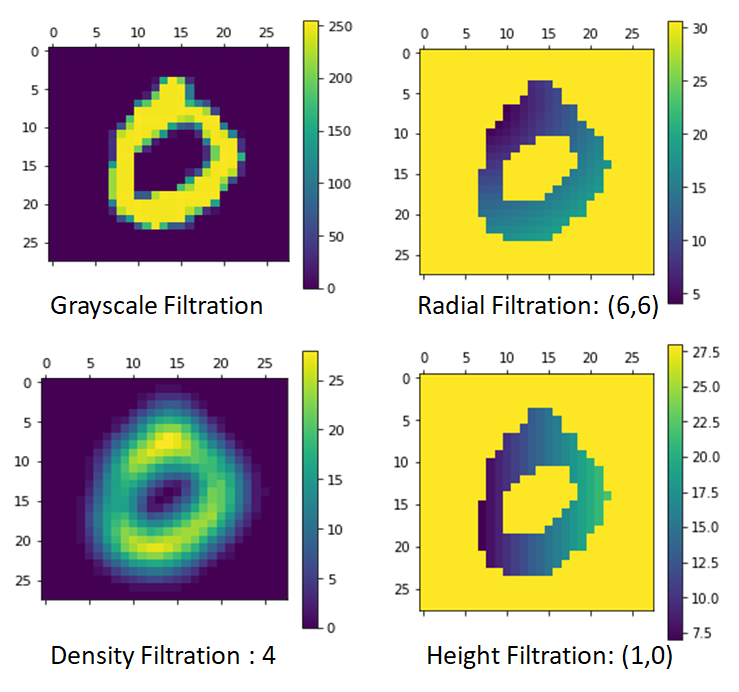
\includegraphics[width=\linewidth,height=0.9\textheight,keepaspectratio]{img1}
\end{center}
\end{frame}

\begin{frame}{5. Topological Pipeline}
Feature vectors are generated by vectorisation of the persistent barcodes obtained from to the persistent homology of the level sets of the filtrations.
\begin{center}
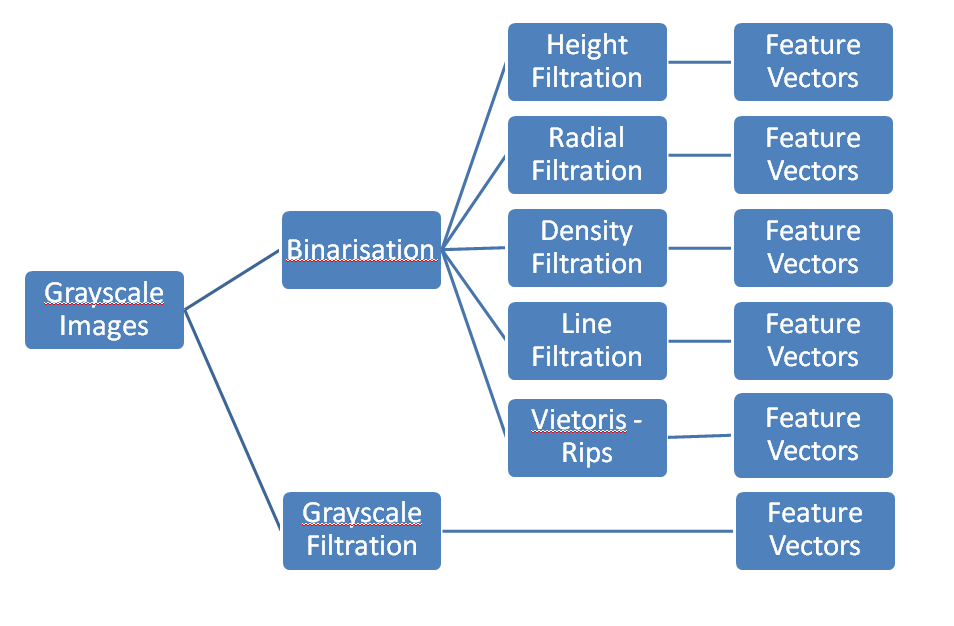
\includegraphics[width=\linewidth,height=0.55\textheight,keepaspectratio]{img2}
\end{center}
\end{frame}

\begin{frame}{6. MNIST Classification}
\begin{center}
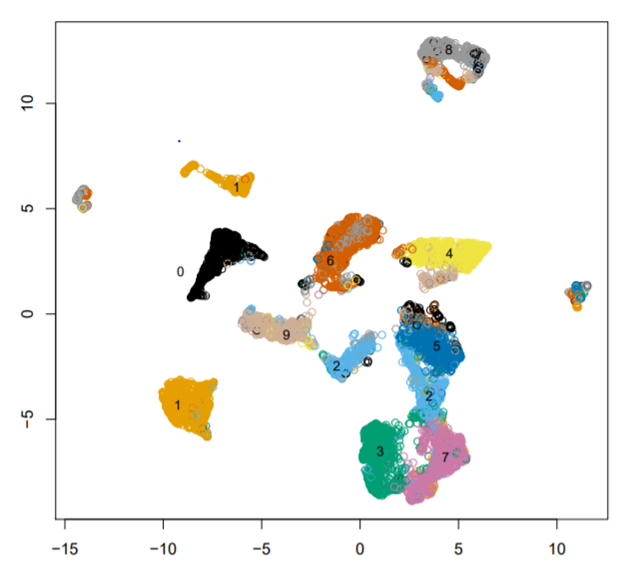
\includegraphics[width=\linewidth,height=0.68\textheight,keepaspectratio]{img3}
\end{center}
UMAP plot of dimension 2 of the 52 feature vectors generated from the topological  pipeline by considering persistent entropy vectorisation.
\end{frame}

\begin{frame}{6. MNIST Classification (contd.)}
\begin{enumerate}
\item k-NN Classification: Performed with k = 5 on 2 dimensional data obtained by using UMAP on feature vectors.\break
Accuracy : \textbf{90.82}

\item{Random Forest Classifier}: Number of trees = 1000
\begin{center}
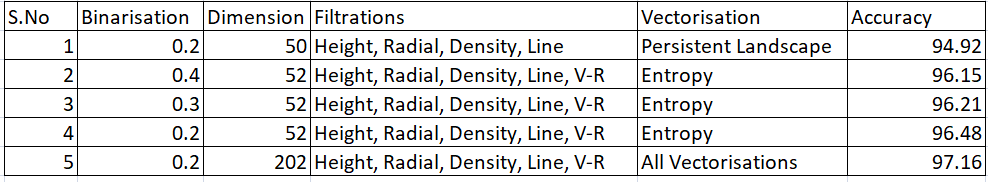
\includegraphics[width=\linewidth,height=3\textheight,keepaspectratio]{img4}
\end{center}
\end{enumerate}

\end{frame}

\begin{frame}{7. Fashion MNIST and Other Datasets}
\begin{center}
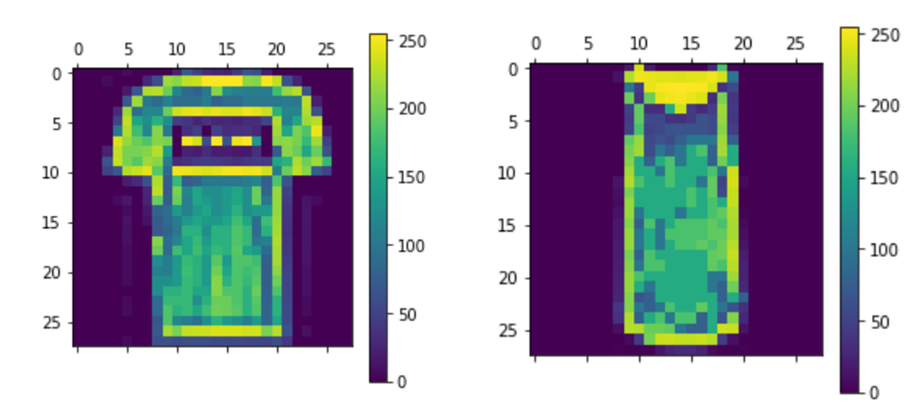
\includegraphics[width=\linewidth,height=0.8\textheight,keepaspectratio]{img7}
\end{center}
Using 200 feature vectors generated by considering all four vectorisations and height, radial, density and line filtrations of the topological pipeline, an accuracy of \textbf{82.85} was obtained on the Fashion MNIST dataset.
\end{frame}

\begin{frame}{7. Fashion MNIST and Other Datasets (contd.)}
Retina Fundus Images:
\begin{center}
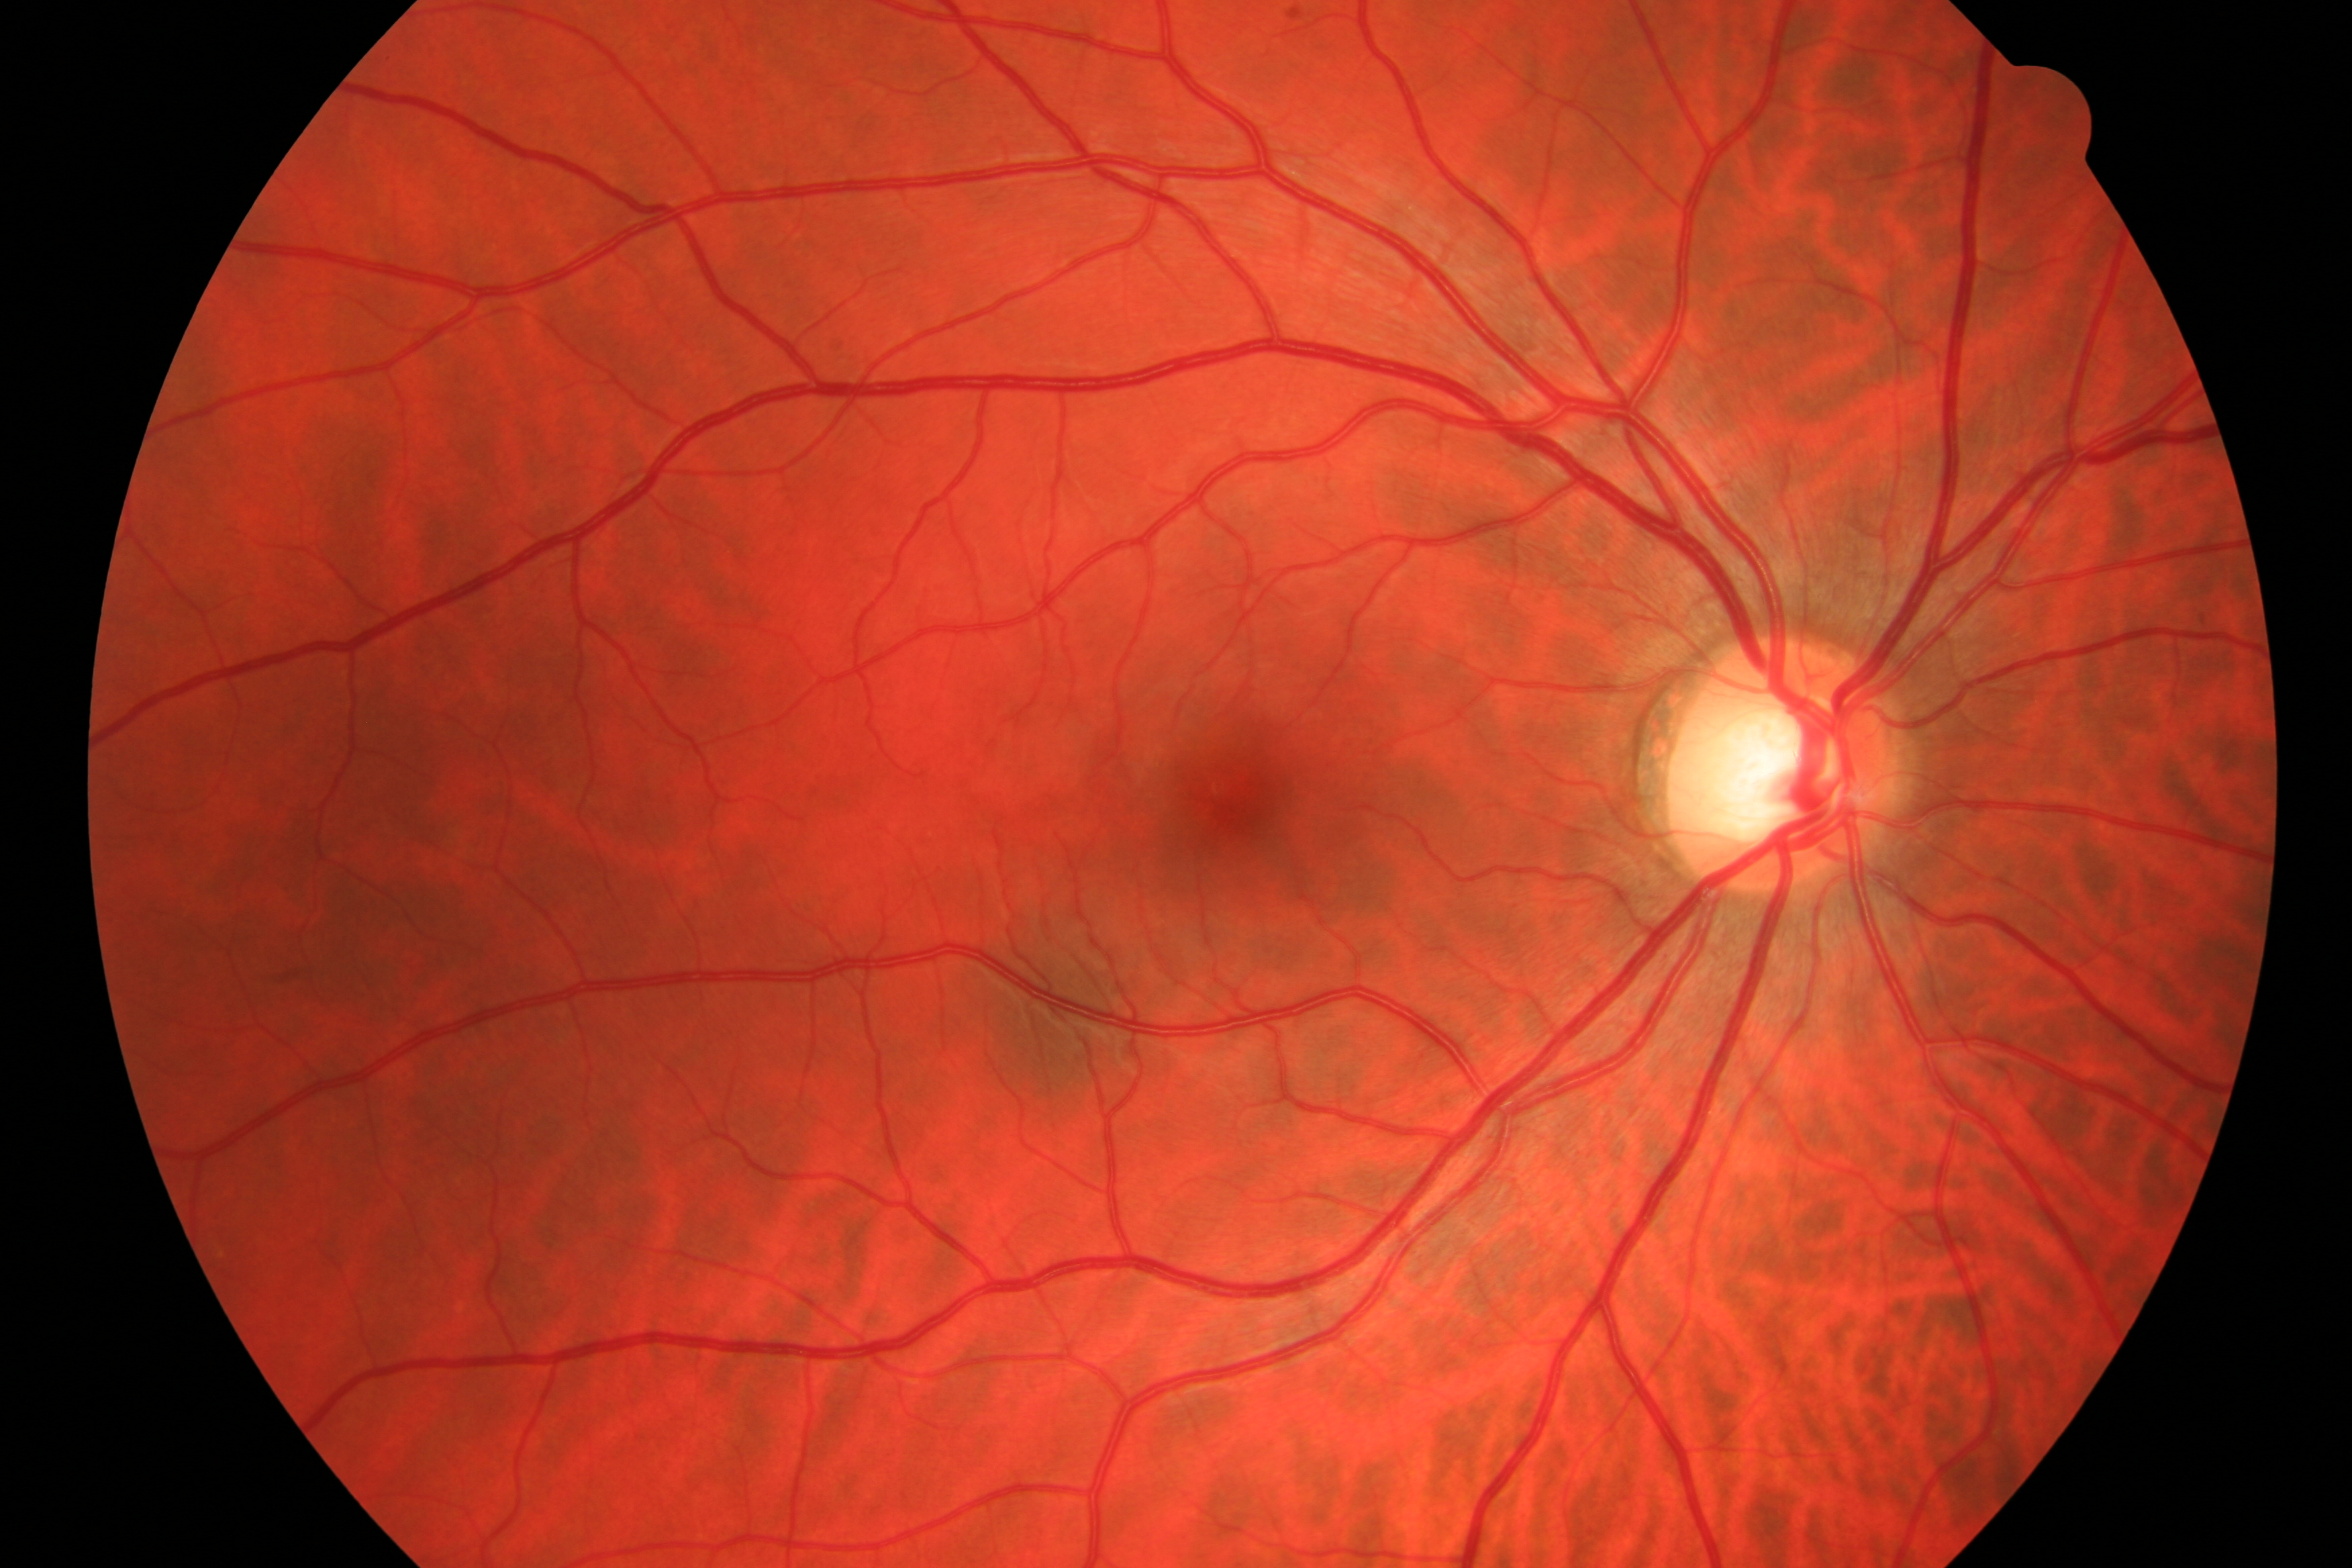
\includegraphics[width=\linewidth,height=.35\textheight,keepaspectratio]{img5}
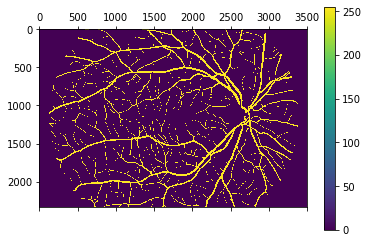
\includegraphics[width=\linewidth,height=.50\textheight,keepaspectratio]{img6}
\end{center}
\end{frame}

\begin{frame}{8. References}
\noindent [1] R. Ghrist, Barcodes: The persistent topology of data \\

[2]. A. Garin and G. Tauzin,”A Topological “Reading” Lesson: Classification of
MNIST using TDA”, https://arxiv.org/pdf/1910.08345.pdf

\end{frame}
\end{document}
